\documentclass[journal,12pt,twocolumn]{IEEEtran}

\usepackage{setspace}
\usepackage{gensymb}

\singlespacing


\usepackage[cmex10]{amsmath}

\usepackage{amsthm}

\usepackage{mathrsfs}
\usepackage{txfonts}
\usepackage{stfloats}
\usepackage{bm}
\usepackage{cite}
\usepackage{cases}
\usepackage{subfig}

\usepackage{longtable}
\usepackage{multirow}

\usepackage{enumitem}
\usepackage{mathtools}
\usepackage{steinmetz}
\usepackage{tikz}
\usepackage{circuitikz}
\usepackage{verbatim}
\usepackage{tfrupee}
\usepackage[breaklinks=true]{hyperref}

\usepackage{tkz-euclide}

\usetikzlibrary{calc,math}
\usepackage{listings}
    \usepackage{color}                                            %%
    \usepackage{array}                                            %%
    \usepackage{longtable}                                        %%
    \usepackage{calc}                                             %%
    \usepackage{multirow}                                         %%
    \usepackage{hhline}                                           %%
    \usepackage{ifthen}                                           %%
    \usepackage{lscape}     
\usepackage{multicol}
\usepackage{chngcntr}

\DeclareMathOperator*{\Res}{Res}

\renewcommand\thesection{\arabic{section}}
\renewcommand\thesubsection{\thesection.\arabic{subsection}}
\renewcommand\thesubsubsection{\thesubsection.\arabic{subsubsection}}

\renewcommand\thesectiondis{\arabic{section}}
\renewcommand\thesubsectiondis{\thesectiondis.\arabic{subsection}}
\renewcommand\thesubsubsectiondis{\thesubsectiondis.\arabic{subsubsection}}


\hyphenation{op-tical net-works semi-conduc-tor}
\def\inputGnumericTable{}                                 %%

\lstset{
%language=C,
frame=single, 
breaklines=true,
columns=fullflexible
}
\begin{document}


\newtheorem{theorem}{Theorem}[section]
\newtheorem{problem}{Problem}
\newtheorem{proposition}{Proposition}[section]
\newtheorem{lemma}{Lemma}[section]
\newtheorem{corollary}[theorem]{Corollary}
\newtheorem{example}{Example}[section]
\newtheorem{definition}[problem]{Definition}

\newcommand{\BEQA}{\begin{eqnarray}}
\newcommand{\EEQA}{\end{eqnarray}}
\newcommand{\define}{\stackrel{\triangle}{=}}
\bibliographystyle{IEEEtran}

\providecommand{\mbf}{\mathbf}
\providecommand{\pr}[1]{\ensuremath{\Pr\left(#1\right)}}
\providecommand{\qfunc}[1]{\ensuremath{Q\left(#1\right)}}
\providecommand{\sbrak}[1]{\ensuremath{{}\left[#1\right]}}
\providecommand{\lsbrak}[1]{\ensuremath{{}\left[#1\right.}}
\providecommand{\rsbrak}[1]{\ensuremath{{}\left.#1\right]}}
\providecommand{\brak}[1]{\ensuremath{\left(#1\right)}}
\providecommand{\lbrak}[1]{\ensuremath{\left(#1\right.}}
\providecommand{\rbrak}[1]{\ensuremath{\left.#1\right)}}
\providecommand{\cbrak}[1]{\ensuremath{\left\{#1\right\}}}
\providecommand{\lcbrak}[1]{\ensuremath{\left\{#1\right.}}
\providecommand{\rcbrak}[1]{\ensuremath{\left.#1\right\}}}
\theoremstyle{remark}
\newtheorem{rem}{Remark}
\newcommand{\sgn}{\mathop{\mathrm{sgn}}}
\providecommand{\abs}[1]{\left\vert#1\right\vert}
\providecommand{\res}[1]{\Res\displaylimits_{#1}} 
\providecommand{\norm}[1]{\left\lVert#1\right\rVert}
%\providecommand{\norm}[1]{\lVert#1\rVert}
\providecommand{\mtx}[1]{\mathbf{#1}}
\providecommand{\mean}[1]{E\left[ #1 \right]}
\providecommand{\fourier}{\overset{\mathcal{F}}{ \rightleftharpoons}}
%\providecommand{\hilbert}{\overset{\mathcal{H}}{ \rightleftharpoons}}
\providecommand{\system}{\overset{\mathcal{H}}{ \longleftrightarrow}}
	%\newcommand{\solution}[2]{\textbf{Solution:}{#1}}
\newcommand{\solution}{\noindent \textbf{Solution: }}
\newcommand{\cosec}{\,\text{cosec}\,}
\providecommand{\dec}[2]{\ensuremath{\overset{#1}{\underset{#2}{\gtrless}}}}
\newcommand{\myvec}[1]{\ensuremath{\begin{pmatrix}#1\end{pmatrix}}}
\newcommand{\mydet}[1]{\ensuremath{\begin{vmatrix}#1\end{vmatrix}}}

\numberwithin{equation}{subsection}

\makeatletter
\@addtoreset{figure}{problem}
\makeatother
\let\StandardTheFigure\thefigure
\let\vec\mathbf

\renewcommand{\thefigure}{\theproblem}

\def\putbox#1#2#3{\makebox[0in][l]{\makebox[#1][l]{}\raisebox{\baselineskip}[0in][0in]{\raisebox{#2}[0in][0in]{#3}}}}
     \def\rightbox#1{\makebox[0in][r]{#1}}
     \def\centbox#1{\makebox[0in]{#1}}
     \def\topbox#1{\raisebox{-\baselineskip}[0in][0in]{#1}}
     \def\midbox#1{\raisebox{-0.5\baselineskip}[0in][0in]{#1}}
\vspace{3cm}
\title{Assignment 8}
\author{Sri Harsha CH}

\maketitle
\newpage

\bigskip
\renewcommand{\thefigure}{\theenumi}
\renewcommand{\thetable}{\theenumi}

\begin{abstract}
This document explains the concept of affine transformation.
\end{abstract}

Download all python codes from 
\begin{lstlisting}
https://github.com/harshachinta/EE5609-Matrix-Theory/tree/master/Assignments/Assignment8/code
\end{lstlisting}
%
and latex-tikz codes from 
%
\begin{lstlisting}
https://github.com/harshachinta/EE5609-Matrix-Theory/tree/master/Assignments/Assignment8
\end{lstlisting}
%
\section{Problem}
To what point must the origin be moved in order that the equation
\begin{align}
    \vec{x}^T\myvec{1 & 2\\2 & -2}\vec{x}+\myvec{10 & -4}\vec{x}=0 \label{eq:q1}
\end{align}
may become
\begin{align}
    \vec{x}^T\myvec{1 & 2\\2 & -2}\vec{x}=1\label{eq:q2}
\end{align}
and through what angle must the axes be turned in order to obtain
\begin{align}
    \vec{x}^T\myvec{p & 0\\0 & q}\vec{x}=1\label{eq:q3}
\end{align}
\section{Explanation}




The general second order equation can be expressed as follows,
\begin{align}
\vec{x^T}\vec{V}\vec{x}+2\vec{u^T}\vec{x}+f=0\label{eq1}
\end{align}
Comparing \eqref{eq:q1} with \eqref{eq:eq1},
\begin{align}
\vec{V} &= \myvec{1 & 2\\2 & -2}\\
\vec{u} &= \myvec{5\\ -2}\\
f &= 0
\end{align}
Let the point to which the origin is moved be $\vec{c}$\\
The above equation \eqref{eq:eq1} can be modified as
\begin{align}
(\vec{x}+\vec{c})^T\vec{V}(\vec{x}+\vec{c})+2\vec{u}^T(\vec{x}+\vec{c})&=0\label{eq:eq2}
\end{align}
From equation \eqref{eq:eq2} consider,
\begin{align}
    &\implies(\vec{x}+\vec{c})^T\vec{V}(\vec{x}+\vec{c})\\
    &\implies\vec{x}^T\vec{V}\vec{x}+\vec{c}^T\vec{V}\vec{x}+\vec{x}^T\vec{V}\vec{c}+\vec{c}^T\vec{V}\vec{c}\label{eq:eq3}\\
    &\implies\vec{x}^T\vec{V}\vec{x}+2\vec{c}^T\vec{V}\vec{x}+\vec{c}^T\vec{V}\vec{c}\label{eq:eq4}
\end{align}
Substituting \eqref{eq:eq4} in equation \eqref{eq:eq2}
\begin{align}
    &\implies\vec{x}^T\vec{V}\vec{x}+2\vec{c}^T\vec{V}\vec{x}+\vec{c}^T\vec{V}\vec{c}+2\vec{u}^T(\vec{x}+\vec{c})=0 \label{eq:eq5}
\end{align}
Comparing equations \eqref{eq:eq5} and \eqref{eq:q2}, we can write as,
\begin{align}
    &\implies 2\vec{c}^T\vec{V}\vec{x}+2\vec{u}^T\vec{x}=0\\
    &\implies \vec{c}^T\vec{V}= -\vec{u}^T\\
    &\implies \vec{c}= -\vec{V}^{-1}\vec{u}= -\myvec{\frac{1}{3}&\frac{1}{3}\\ \frac{1}{3}&-\frac{1}{6}}\myvec{5\\-2} \label{eq:eq6}\\
    &\implies \boxed{\vec{c}= \myvec{-1\\-2}} \label{eq:eq7}
\end{align}
From \eqref{eq:eq7}, when the origin is moved to point $\vec{c}$, the equation \eqref{eq:q1} becomes \eqref{eq:q2}.\\
\\
From equations \eqref{eq:q1} and \eqref{eq:eq7}, $\vec{V}$ doesn't change
\begin{align}
    \det(\vec{V})&=-6
\end{align}
Since $\det(\vec{V})<0$ the given equation represents the hyperbola\\
\\
From equation \eqref{eq:q2}, the equation is of the form,
\begin{align}
    \vec{x}^T\vec{V}\vec{x}+f=0
\end{align}
The matrix $\vec{V}$ can be decomposed as,
\begin{align}
    \vec{V} = \vec{P}\vec{D}\vec{P}^T \quad \vec{D}=\myvec{\lambda_1&0\\0&\lambda_2}
\end{align}
where $\lambda_1$ and $\lambda_2$ are Eigen values of $\vec{V}$, and $\vec{P}$ contains the Eigen vectors corresponding to the Eigen values $\lambda_1$ and $\lambda_2$. The affine transformation is given by,
\begin{align}
    \vec{x} = \vec{P}\vec{y}+\vec{c}
\end{align}
where, $\vec{P}$ indicates the rotation of axes and $\vec{c}$ indicates the shift of origin.\\
Eigen values of $\vec{V}$ are,
\begin{align}
   \mydet{\lambda\vec{I}-\vec{v}}=0\\
    \implies \mydet{\lambda-1&-2\\-2&\lambda+2}=0\\
    \implies \lambda^2+\lambda-6=0\\
    \implies \lambda_1=-3,\lambda_2=2\\
    \vec{D}=\myvec{-3&0\\0&2}
\end{align}
Eigen vector for $\lambda_1$=-3,
\begin{align}
    \lambda_1\vec{I}-\vec{v}=\myvec{-4&-2\\-2&-1}\xleftrightarrow[]{R_2\leftarrow R_2-\frac{R_1}{2}}\myvec{-2&-1\\0&0}\\
    \implies \vec{P_1}=\myvec{1\\-2}=\myvec{\frac{1}{\sqrt{5}}\\\frac{-2}{\sqrt{5}}}
\end{align}
Eigen vector for $\lambda_2$=2,
\begin{align}
    \lambda_1\vec{I}-\vec{v}=\myvec{1&-2\\-2&4}\xleftrightarrow[]{R_2\leftarrow R_2+2R_1}\myvec{1&-2\\0&0}\\
    \implies \vec{P_2}=\myvec{2\\1}=\myvec{\frac{2}{\sqrt{5}}\\\frac{1}{\sqrt{5}}}
\end{align}
\begin{align}
    \vec{P} = \myvec{\frac{1}{\sqrt{5}}&\frac{2}{\sqrt{5}}\\\frac{-2}{\sqrt{5}}&\frac{1}{\sqrt{5}}} \label{eq:eq15}
\end{align}
Therefore $\vec{V}$ can be written as,
\begin{align}
    \vec{V}=\myvec{\frac{1}{\sqrt{5}}&\frac{2}{\sqrt{5}}\\\frac{-2}{\sqrt{5}}&\frac{1}{\sqrt{5}}}\myvec{-3&0\\0&2}\myvec{\frac{1}{\sqrt{5}}&\frac{-2}{\sqrt{5}}\\\frac{2}{\sqrt{5}}&\frac{1}{\sqrt{5}}}
\end{align}
Equation \eqref{eq:q2} can be written as,
\begin{align}
    \vec{x}^T\left[\myvec{\frac{1}{\sqrt{5}}&\frac{2}{\sqrt{5}}\\\frac{-2}{\sqrt{5}}&\frac{1}{\sqrt{5}}}\myvec{-3&0\\0&2}\myvec{\frac{1}{\sqrt{5}}&\frac{-2}{\sqrt{5}}\\\frac{2}{\sqrt{5}}&\frac{1}{\sqrt{5}}}\right]\vec{x}=1\\
  \left[\myvec{\frac{1}{\sqrt{5}}&\frac{-2}{\sqrt{5}}\\\frac{2}{\sqrt{5}}&\frac{1}{\sqrt{5}}}\vec{x}\right]^T\myvec{-3&0\\0&2}\left[\myvec{\frac{1}{\sqrt{5}}&\frac{-2}{\sqrt{5}}\\\frac{2}{\sqrt{5}}&\frac{1}{\sqrt{5}}}\vec{x}\right]= 1\label{eq:eq11}
\end{align}
Consider the rotation transformation 
\begin{align}
  \vec{x}=\vec{P}\vec{y}\\
  \implies \vec{x}=\myvec{\frac{1}{\sqrt{5}}&\frac{2}{\sqrt{5}}\\\frac{-2}{\sqrt{5}}&\frac{1}{\sqrt{5}}}\vec{y}\label{eq:eq12}\\
  \vec{P}^{-1}\vec{x}=\vec{P}^{-1}\vec{P}\vec{y}\\
  \implies \vec{y}= \vec{P}^{-1}\vec{x}\\
  \text{But, }\vec{P}^{-1}=\vec{P}^T\\
  \implies \vec{y}=\myvec{\frac{1}{\sqrt{5}}&\frac{-2}{\sqrt{5}}\\\frac{2}{\sqrt{5}}&\frac{1}{\sqrt{5}}}\vec{x} \label{eq:eq12}
\end{align}
Using \eqref{eq:eq12} in \eqref{eq:eq11}, the equation can be rewritten as
\begin{align}
     \vec{y}^T\myvec{-3&0\\0&2}\vec{y}=1 \label{eq:eq13}
\end{align}
Equation \eqref{eq:eq13} is same as \eqref{eq:q3} with $p$=-3 and $q$=2.\\
From equation \eqref{eq:eq15}, the orthogonal matrix represents the rotation matrix in form of,
\begin{align}
    \vec{P}=\myvec{\cos\theta & \sin\theta\\ -\sin\theta& \cos\theta} \label{eq:eq16}
\end{align}
Comparing \eqref{eq:eq15} and \eqref{eq:eq16},
\begin{align}
    \cos\theta = \frac{1}{\sqrt{5}}\\
    \implies \boxed{\theta = 63.43^{\circ}}
\end{align}
From equation \eqref{eq:eq16},if the axes is turned by $\theta$ then the equation obtained would be \eqref{eq:q3}.
\renewcommand{\thefigure}{\arabic{figure}}
\begin{figure}[h!]
	\centering
	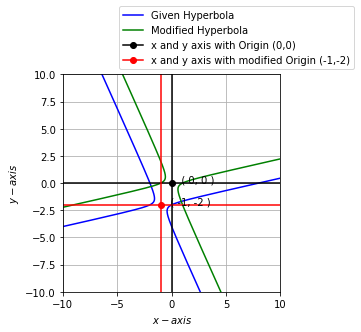
\includegraphics[width=\columnwidth]{hyperbola1.png}
	\caption{Hyperbola plot when origin is shifted}
	\label{myfig}
\end{figure}
\\\end{document}
